\documentclass[10pt,a4paper]{article}

% ---------------------------------------------------------------------------
% Chronicle -- video-free memory (VFM) architecture
% Compile: pdflatex VFM_ARCHITECTURE.tex (twice)
% ---------------------------------------------------------------------------

\usepackage[T1]{fontenc}
\usepackage[utf8]{inputenc}
\usepackage{lmodern}
\usepackage[margin=1.8cm,top=1.65cm,bottom=1.65cm]{geometry}
\usepackage{microtype}
\usepackage{xcolor}
\usepackage{booktabs}
\usepackage{tabularx}
\usepackage{array}
\usepackage{enumitem}
\usepackage{titlesec}
\usepackage{fancyhdr}
\usepackage{amsmath,amssymb}
\usepackage{tikz}
\usetikzlibrary{arrows.meta,positioning,fit,backgrounds}
\usepackage[hidelinks]{hyperref}

\definecolor{ink}{HTML}{0F172A}
\definecolor{accent}{HTML}{0F766E}
\definecolor{accent2}{HTML}{1D4ED8}
\definecolor{muted}{HTML}{64748B}
\definecolor{panel}{HTML}{F1F5F9}
\definecolor{warn}{HTML}{B45309}
\definecolor{vlm}{HTML}{7C3AED}

\color{ink}
\setlength{\headheight}{19pt}
\setlength{\parindent}{0pt}
\setlength{\parskip}{4pt}
\setlength{\emergencystretch}{2em}
\renewcommand{\arraystretch}{1.16}

\titleformat{\section}{\large\bfseries\color{accent}}{\thesection}{0.6em}{}
\titleformat{\subsection}{\normalsize\bfseries\color{accent2}}{\thesubsection}{0.5em}{}
\titlespacing*{\section}{0pt}{10pt}{4pt}
\titlespacing*{\subsection}{0pt}{7pt}{2pt}

\pagestyle{fancy}
\fancyhf{}
\fancyhead[L]{\footnotesize\color{muted}Chronicle --- video-free memory architecture}
\fancyhead[R]{\footnotesize\color{muted}October 2026}
\fancyfoot[C]{\footnotesize\color{muted}\thepage}
\renewcommand{\headrulewidth}{0.2pt}
\renewcommand{\headrule}{\hbox to\headwidth{\color{panel}\leaders\hrule height \headrulewidth\hfill}}

\newcommand{\code}[1]{\texttt{\small #1}}
\newcommand{\kw}[1]{\textcolor{accent2}{\textbf{#1}}}
\newcommand{\vlm}[1]{\textcolor{vlm}{\textbf{#1}}}
\newcommand{\panel}[1]{%
  \noindent\colorbox{panel}{%
    \begin{minipage}{\dimexpr\linewidth-2\fboxsep\relax}
    \vspace{2pt}#1\vspace{2pt}
    \end{minipage}}%
}

\begin{document}

\begin{center}
{\LARGE\bfseries Chronicle}\\[2pt]
{\Large Video-free memory (VFM) architecture}\\[6pt]
{\color{muted}\small Technical note --- 27 October 2026}\\[2pt]
{\color{muted}\small Branch \code{experiment/video-free-memory} --- main UI + VLM-first answers}
\end{center}

\vspace{-2pt}
\panel{
\textbf{One-sentence summary.} Chronicle compiles a video episode \emph{once} into a compact,
timestamped memory --- VLM captions, a salience-coalesced event ledger, a few WebP evidence
frames and an LLM-ready pack --- then answers questions from that memory in microseconds, with no
video and no video model in the query path. The zine dashboard from \code{main} is the UI; the VLM
memory is the answer engine.
}

\section{What is different from the graph-only dashboard}

The \code{main} dashboard replays a live graph: entities, state transitions, spatial edges and
zones. That is excellent for visual inspection, but it has two limitations for question answering:

\begin{itemize}[leftmargin=1.25em,itemsep=1pt]
  \item It only knows what the graph recorded. Replay clips often have \textbf{state/edge events
        but no VLM interaction table}, so ``what happened around 10\,s?'' had no semantic answer.
  \item Labels can arrive late. If an entity row is emitted at \code{last\_seen}, the first half of
        the episode shows anonymous \code{Track} rows.
\end{itemize}

VFM adds the layer the graph does not keep: \vlm{dense natural-language captions} at 30\,s
resolution, a compact event ledger derived from the graph, evidence snapshots, and a retrieval
engine whose answers are deterministic. The graph remains the index; the captions and events are
the recallable memory.

\section{Architecture at a glance}

\begin{center}
\begin{tikzpicture}[
  node distance=5mm and 7mm,
  box/.style={draw=ink!55, rounded corners=2pt, fill=white, align=center,
              font=\scriptsize, inner sep=4pt, minimum height=9mm},
  vbox/.style={box, draw=vlm!70, fill=vlm!6},
  sbox/.style={box, draw=accent!70, fill=accent!6},
  arr/.style={-{Latex[length=2mm]}, draw=ink!65, thick},
]
\node[vbox] (video) {video / graph DB\\\scriptsize (bundled clip, upload, pipeline)};
\node[vbox, right=of video] (vlm) {VLM captioner\\\scriptsize 30\,s windows, 3 frames};
\node[sbox, right=of vlm] (ledger) {caption ledger\\\scriptsize zlib JSON, objects/actions/tags};
\node[box, below=of video] (graph) {graph event source\\\scriptsize entities, states, edges, zones};
\node[sbox, right=of graph] (events) {event ledger\\\scriptsize salience coalescing, 17\,B/event};
\node[sbox, right=of events] (vault) {SQLite vault\\\scriptsize packed events + strings + meta};
\node[box, below=of graph] (evidence) {evidence snapshots\\\scriptsize 480\,px WebP q75};
\node[box, right=of evidence] (pack) {memory pack\\\scriptsize 2k/4k/8k token ceilings};
\node[box, right=of pack] (query) {deterministic query\\\scriptsize intents + cache + counts};
\node[box, below=of evidence] (ui) {zine UI (main)\\\scriptsize Memory card, chat, screenshots};
\node[box, right=of ui] (qwen) {optional Qwen\\\scriptsize phrasing over the pack only};
\node[box, right=of qwen] (answer) {answer + citations\\\scriptsize + evidence frame + PNG};

\draw[arr] (video) -- (vlm);
\draw[arr] (vlm) -- (ledger);
\draw[arr] (graph) -- (events);
\draw[arr] (events) -- (vault);
\draw[arr] (video) -- (evidence);
\draw[arr] (ledger) -- (vault);
\draw[arr] (vault) -- (query);
\draw[arr] (pack) -- (query);
\draw[arr] (query) -- (answer);
\draw[arr] (qwen) -- (answer);
\draw[arr] (query) -- (ui);
\draw[arr] (ui) -- (qwen);
\end{tikzpicture}
\end{center}

\noindent
The two inputs are compiled in parallel and joined in the vault. Query time reads only the vault
and the pack. The source video is retained for playback and screenshot capture, but is never
required to answer a question.


\section{Glossary: what the terms mean}

\begin{center}
\small
\begin{tabularx}{\linewidth}{@{}l X@{}}
\toprule
\textbf{Term} & \textbf{Meaning in Chronicle} \\
\midrule
VFM & \textbf{Video-Free Memory}. The compiled artefact that answers questions without the source video: packed events, captions, evidence references and metadata. \\
VLM & Vision-language model. Used \emph{once at compile time} to caption frames/windows (default \code{qwen2.5vl:3b}); not used for deterministic answers. \\
Graph DB & The live per-episode SQLite graph: entities, states, edges, zones, anchors and observations. Source of truth for identity, state and counts. \\
Vault & The compact SQLite file written by the compiler: struct-of-arrays events, string dictionary, captions, evidence index and metadata. \\
Caption ledger & zlib-compressed JSON of 30\,s (or 20\,s) windows. Each window has a caption, objects, actions, zone, tags and 3 timestamped frame captions. \\
Event ledger & Salience-coalesced state/edge/interaction events from the graph. Packed at about 17 bytes/event. \\
Salience coalescing & Filtering visibility noise (camera pan, occlusion, reacquisition) and merging repeated touches/placements into memory-worthy events. \\
Evidence still & A 480\,px WebP snapshot selected at an interaction, crop, zone keyframe or anchor. Stored with a timestamp and relative path. \\
Memory pack & LLM-ready Markdown/JSON: verified answer + ranked captions/events + evidence references + answering rules. Budgeted at 2k/4k/8k tokens. \\
Deterministic query & Intent + time + entity lookup over the vault. No LLM, no video, no frame sampling; answers carry citations. \\
Track / peak / physical & Track = raw tracker id count (upper bound); peak = most same-label tracks visible in one frame (lower bound); physical = tracks after cross-label duplicate and transient removal (estimate). \\
Auto-compile & Building the vault once on first view of a clip, in the background. Query stays on the graph fallback until it is ready. \\
Frame chip & The per-answer \code{frame @ t} control: seek to the cited time, capture that frame, open it in a save/fullscreen lightbox. \\
Graph fallback & If VFM has no answer, the same chat asks the live graph engine and labels the answer \code{graph-fallback}. \\
\bottomrule
\end{tabularx}
\end{center}

\section{End-to-end workflow}

\subsection*{A. Graph-backed clip (bundled / ingested run)}

\begin{enumerate}[leftmargin=1.35em,itemsep=1pt]
  \item \textbf{Ingest.} Perception writes entities, state transitions, edges, anchors, zones and observations into an episode DB. The graph state machine emits a transition per meaningful change.
  \item \textbf{Verify important actions.} Interaction clips are queued; a temporal strip (pre/contact/post) is built and the action verifier (Florence-2 path) returns an action, confidence and rejection reason. Low-confidence/rejected clips stay in the review queue.
  \item \textbf{Compile (on first view or via the button).} The service snapshots the DB, captions the video once, builds the salience event ledger, writes the vault, extracts evidence stills, renders \code{memory.html}, writes the memory pack and zips the downloads.
  \item \textbf{Answer.} The zine chat routes to the vault. A question resolves an intent (where / when / around / before / after / count / holding / inventory / yes-no), looks up captions/events/time and returns an answer with citations and an evidence reference.
  \item \textbf{Inspect.} The answer shows citation chips, a \code{frame @ t} button, an evidence thumbnail only when the still is within 8\,s of the question, and the graph fallback if the vault has no match.
  \item \textbf{Export / import.} Export writes one ZIP with the full current timeline, snapshot, CSVs, all replay timelines and the VFM artefacts; import reloads a timeline without re-ingesting video.
\end{enumerate}

\subsection*{B. Caption-first clip (fresh upload / long street walk, no DB)}

\begin{enumerate}[leftmargin=1.35em,itemsep=1pt]
  \item \textbf{Upload / select} the video. No perception DB is required.
  \item \textbf{Caption once:} 30\,s windows (20\,s for short clips), 3 frames each. A window caption and per-frame captions become the ledger; objects/actions become coarse entities and \code{SEEN} events.
  \item \textbf{Build the caption vault, evidence and pack} with the same compiler stages.
  \item \textbf{Answer} from the caption/event ledger. Counts are caption coverage, not physical counts; the UI says so.
  \item \textbf{Inspect / export} exactly as in the graph-backed path.
\end{enumerate}

\begin{center}
\small
\begin{tabularx}{\linewidth}{@{}l r r r@{}}
\toprule
Episode & Duration & Compile (once) & Deterministic query p50 \\
\midrule
Synthetic demo & 12\,s & $\sim$12\,s & 0.05--0.06\,ms \\
Aria walk & 60\,s & $\sim$20\,s & 0.05--0.06\,ms \\
London walk & 15\,min & $\sim$5\,min & 0.89\,ms (cold), 3\,ms cache \\
\bottomrule
\end{tabularx}
\end{center}

\section{What is saved now (more than the graph)}

The graph is still saved. VFM adds four new artefacts. All of them are derived once, compressed,
and stored next to the source run; the video itself is optional at query time.

\begin{center}
\small
\begin{tabularx}{\linewidth}{@{}l X r r@{}}
\toprule
\textbf{Artefact} & \textbf{What it contains} & \textbf{Demo} & \textbf{Walking} \\
\midrule
Graph DB & entities, states, edges, zones, observations (source of truth) & 168\,KB & 254\,KB \\
Packed vault & struct-of-arrays events, string dictionary, metadata, answer cache & 28.7\,KB & 31.7\,KB \\
Caption ledger & 30\,s VLM windows: caption, objects, actions, zone, tags, 3 frame captions & 1 window & 2 windows \\
Event ledger & salience-coalesced state/edge/interaction events & 8 events & 11 events \\
Evidence & 480\,px WebP stills, ranked by interaction / crop / zone keyframe & 8 frames & 8 frames \\
Memory pack & verified answer + ranked captions/events + evidence refs + rules & 2.4\,KB & 3.0\,KB \\
Report & single-file offline HTML with timeline, captions, query box & 366\,KB & 410\,KB \\
\midrule
\textbf{Whole job dir} & vault + ledger + evidence + report + pack + zip & \textbf{988\,KB} & \textbf{1.3\,MB} \\
\bottomrule
\end{tabularx}
\end{center}

\noindent
The report and zip duplicate bytes for convenience; the \emph{at-rest memory} is the vault +
ledger + evidence. On a 60-minute synthetic episode (2{,}474 events, 184 caption windows, 40
snapshots) the vault is 142\,KB and the whole memory stays far below the source video.

\subsection{Why this is more information}

\begin{itemize}[leftmargin=1.25em,itemsep=1pt]
  \item \textbf{Semantics.} The graph knows \code{person VISIBLE\_MOVING}; the caption knows
        ``a person walks on a sidewalk holding a cup of coffee''. The second is what a user asks
        for.
  \item \textbf{Coverage.} Captions cover the whole episode, including segments where the tracker
        emitted no interaction row.
  \item \textbf{Recall by time.} Caption windows are timestamped, so ``around 10\,s'' is a range
        query, not a similarity search over one frame.
  \item \textbf{Evidence.} Answers point to stored stills, so the UI can show the frame and seek
        the video without re-ingesting.
  \item \textbf{Counts.} Compile-time observations also yield track counts, peak simultaneous
        visibility, and cross-label duplicate merges (Section~\ref{sec:counts}).
\end{itemize}

\subsection{Design lineage}

The design deliberately borrows one idea from each line of work: caption-first episodic QA
\cite{capmem}, time as a first-class key \cite{egocite}, query-agnostic high-recall memory
\cite{merit}, egocentric entity/event schemas \cite{egograph,vlkng,r4dsg}, graph retrieval
\cite{hipporag}, tiered sensory/short/long-term memory \cite{lightmem}, event segmentation
\cite{emllm}, bounded retention \cite{videomem}, text-first / frames-on-demand \cite{focusgraph,captiononce},
semantic answer caching \cite{semcache}, and personal-memory retrieval \cite{egomemory}. The
model-native memory work (Titans, MemoryLLM) \cite{titans,memoryllm} is a north star, not a
dependency.

\section{Compile pipeline}

\begin{enumerate}[leftmargin=1.35em,itemsep=1pt]
  \item \textbf{Snapshot the source DB.} SQLite's backup API makes a consistent copy while the
        ingest worker may still be writing.
  \item \textbf{Caption once.} Split the video into 30\,s windows; sample three frames per window;
        caption each frame with a VLM (\code{qwen2.5vl:3b} by default) and synthesise a window
        caption. Store zlib-compressed JSON with objects, actions, zone and tags.
  \item \textbf{Build the event ledger.} Read entities, state transitions, anchors and edges;
        coalesce visibility noise and repeated touches into salient events. Pack them
        struct-of-arrays at roughly 17 bytes/event.
  \item \textbf{Build the vault.} Write 1\,KB SQLite pages, the string dictionary, packed events,
        captions and metadata (including per-label count summaries).
  \item \textbf{Extract evidence.} Save a bounded set of 480\,px WebP q75 stills (interaction
        strips, object crops, zone keyframes). No full-resolution frames are retained.
  \item \textbf{Render the report.} Write a single-file HTML with the timeline, captions and a
        client-side query box; embed evidence as data URLs.
  \item \textbf{Write the pack.} Produce an LLM-ready Markdown/JSON pack. Budgets of 2k/4k/8k
        tokens keep the verified answer and rules, then add windows/events until the ceiling.
  \item \textbf{Zip and manifest.} Expose \code{vault.db}, \code{memory.html}, \code{ledger.json},
        \code{memory\_pack.md/json}, CSVs and \code{evidence/}.
\end{enumerate}

\noindent
The compile is the only expensive step (seconds to tens of seconds, dominated by VLM calls). In
the UI it runs \emph{once per clip, in the background}, on first view. After that, opening the clip
or asking a question does not touch the video.

\section{Query path and latency}

\textbf{Deterministic vault.} The query engine resolves an intent (where/when/around/before/after/
count/inventory/yes-no/keyword), looks up entities and events by time, and returns an answer with
citations and an evidence reference. A canonical answer cache makes paraphrases hit the same entry.
No LLM, no video, no frame extraction in this path.

\textbf{Qwen (optional).} The pack is passed to a local text model for phrasing
(\code{qwen2.5:7b-instruct}). The model never sees frames; it sees the verified structured answer,
timestamped captions, events and evidence references. It is an optional polish layer, not a
dependency.

\begin{center}
\small
\begin{tabularx}{\linewidth}{@{}X r r r@{}}
\toprule
Path & Accuracy (30 questions) & p50 & Video at answer time \\
\midrule
Deterministic VFM vault & \textbf{30/30} & \textbf{0.05--0.06\,ms} & no \\
Qwen 7B from memory pack & \textbf{30/30} & 1.07\,s & no \\
Original graph + Qwen 7B & 14/30 & 0.85\,s & yes \\
9-frame contact sheet + Qwen2.5-VL & 7/30 & 4.46\,s & yes (19.24\,MB) \\
\bottomrule
\end{tabularx}
\end{center}

\noindent
The 30-question set is an internal regression suite, not a public benchmark. It is useful because
it covers location, temporal, count, negation, before/after and paraphrase questions on the same
episodes.

\section{Counts: tracks, visibility and duplicates}
\label{sec:counts}

Count questions need more than one number. At compile time we compute, per label:

\begin{center}
\small
\begin{tabularx}{\linewidth}{@{}l X@{}}
\toprule
\textbf{Field} & \textbf{Meaning} \\
\midrule
\code{tracks} & raw number of tracker ids with that label (upper bound) \\
\code{peak} & max same-label tracks present in one observation frame (lower bound) \\
\code{physical} & tracks after removing cross-label duplicate detections and one-frame transients \\
\code{duplicates} & tracks that were near-identical to a track under another label \\
\code{merged\_into} & which label absorbed those duplicates \\
\bottomrule
\end{tabularx}
\end{center}

\noindent
A duplicate is accepted only when two different-label boxes share the same frame with IoU
$\ge 0.90$ and centre distance $\le 5$\,px, and one label has more total observations. This is
deliberately conservative: same-label co-visible boxes on cook have max IoU $\approx 0.01$, so
they are \emph{not} merged.

On the cook clip this turns four ``bowl'' tracks into \textbf{zero physical bowls}: two of the
plates were emitted under both \code{bowl} and \code{plate} (IoU 0.91--0.99), and a fourth track was
a one-frame detection. The plates resolve to two physical plates. On walking, two car tracks are
one object at a time, so the answer is a range (1--2), not a false single count.

\section{Dashboard integration}

The zine mission control from \code{main} is the default UI (\code{./chronicle.sh start}, port
8080 in main, 8082 in this worktree). VFM is added behind it, not as a second uploader:

\begin{itemize}[leftmargin=1.25em,itemsep=1pt]
  \item \textbf{Auto-compile.} On first view of a clip with a graph DB, the vault builds in the
        background. The Memory card shows progress, then report and downloads.
  \item \textbf{VLM-first chat.} Once ready, the existing chat routes to the vault
        (\code{provider: vfm-memory}) and answers in microseconds. If not ready, a state/edge
        fallback still answers ``around $t$'' instead of claiming no interactions exist.
  \item \textbf{Screenshot at answer time.} Every grounded answer gets a frame chip that seeks to
        the citation, captures the exact frame, stamps clip + timestamp, and opens a lightbox.
  \item \textbf{Fullscreen.} Stage toolbar \code{S} (screenshot) and \code{F} (fullscreen); the
        screenshot lightbox has its own fullscreen button.
  \item \textbf{Downloads.} \code{vault.db}, \code{memory.html}, \code{memory\_pack.md},
        \code{memory\_pack.json}, \code{memory.zip}.
\end{itemize}


\section{Event-driven evidence and verification}

The trigger for “something important happened” is the \textbf{graph state machine}, not the captioner. It emits transitions such as \code{NEW}, \code{INTERACTED}, \code{HELD}, \code{CONTAINED}, \code{PLACED\_ON}, \code{LOST}. Those transitions drive two bounded systems:

\begin{itemize}[leftmargin=1.25em,itemsep=1pt]
  \item \textbf{Verification queue.} Interaction clips are de-duplicated, bounded and queued. A temporal strip gives the verifier pre/contact/post frames; the Florence-2 path returns an action primitive, confidence and a rejection reason. Rejected or ambiguous actions are inspectable in the review queue/telemetry.
  \item \textbf{Evidence selection.} At compile time, \code{extract\_evidence.select\_events} picks major markers (\code{INTERACTED}, \code{HELD}, \code{CONTAINED}, \code{LOST}, \code{NEW}, \code{PICK}, \code{PLACE}, \code{INSERT}, anchors/keyframes), enforces a 2\,s minimum gap and a 40-still cap, then writes 480\,px WebP stills with an append-only index.
\end{itemize}

\noindent
The standalone \code{evidence\_recorder.py} prototype can write 640\,px JPEGs plus a JSONL index. The zine pipeline now also includes an \textbf{event-clip recorder}: transition, low-confidence and label-conflict triggers receive a readable salience score, coalesce within 2.5\,s, and become a 3\,s pre + 3\,s post \code{clip.mp4}, a rebased \code{events.jsonl} replay and a \code{graph.json} snapshot (entity/zone/edge nodes at the anchor time). It then extracts \textbf{three frames} (1\,s pre / contact / 1\,s post), sends them to Qwen2.5-VL (or Florence-2 as fallback), appends the verified interaction to the timeline and compiles a small queryable per-event \code{vault.db}; one \code{snapshot.jpg} is retained for audit. A disagreeing VLM answer never overwrites a strong graph state: the disagreement is flagged for review. The \textbf{events} button and \code{POST /api/event-clips} expose the whole bounded path; see \code{docs/EVENT\_CLIPS.md}. There is still \textbf{no learned live anomaly score} and the VLM is not called on every strange moment. That remains a deliberate scope choice: the recorder is bounded, the trigger is auditable, and only selected clips pay the VLM cost.

\noindent
The bounded shape is: transition / low confidence / label conflict $\rightarrow$ salience score $\rightarrow$ 3\,s pre + 3\,s post clip $\rightarrow$ 3 frames to Qwen2.5-VL / Florence-2 on that clip only $\rightarrow$ verified interaction + snapshot + per-event vault. The event-clip recorder implements this path (\code{POST /api/event-clips}); the VLM pass is optional when no model is reachable and falls back to the graph hint plus the rule classifier. This keeps the cost bounded and makes the trigger auditable.

\section{Is this a good system?}

\subsection*{Strengths}

\begin{itemize}[leftmargin=1.25em,itemsep=1pt]
  \item \textbf{Speed and cost}: answers come from a 95\,KB vault, not a 249\,MB video; cold p50 is sub-millisecond to a few milliseconds and repeat answers are cached.
  \item \textbf{Coverage}: captions cover the whole episode, including segments where the tracker emitted no interaction row.
  \item \textbf{Video-free}: after compile, query, report, pack and evidence do not need the video. The source is kept only for playback/screenshots.
  \item \textbf{Evidence and audit}: timestamped citations, stored stills, frame chips, fullscreen and ZIP export.
  \item \textbf{Deterministic}: no model in the default answer path, so it is reproducible and cheap on stage.
  \item \textbf{Composable}: the graph is still the source of identity/state/counts and the fallback when captions have no answer.
\end{itemize}

\subsection*{Where it is weaker}

\begin{itemize}[leftmargin=1.25em,itemsep=1pt]
  \item \textbf{Lossy compression}: captions are a summary; fine-grained motion, small text, audio and subtle social cues are lost.
  \item \textbf{Caption hallucination}: the VLM can misdescribe an object. Evidence and citations make it auditable, not infallible.
  \item \textbf{Counts}: track/peak/physical are estimates, not hand-labelled ground truth for every episode.
  \item \textbf{Long video without a DB}: no graph, so no state/edge fallback and counts are caption coverage only.
  \item \textbf{Internal evaluation}: the 30-question suite is a regression test, not a public benchmark.
\end{itemize}

\noindent
Verdict: it is a \emph{good retrieval-and-recall system}, not a replacement for a full video-reasoning model. It is strongest when the question is “what happened / where / when / how many / what is X holding”, and weakest on “why / exactly how / what did the tiny object do”.

\section{How this compares with common industry approaches}

\begin{center}
\small
\begin{tabularx}{\linewidth}{@{}p{2.25cm} X X X@{}}
\toprule
\textbf{Approach} & \textbf{Answer path} & \textbf{Strength} & \textbf{Weakness} \\
\midrule
Frame-sampling video LLM & Sample N frames per question and send them to a VLM & Open-ended reasoning, no compile step & Re-samples every question; cost/latency scale with length; coverage depends on sampling; video must be available \\
Long-video RAG / frame retrieval & Embed frames/clips, retrieve top-$k$ per question, then VLM & Better coverage than fixed sampling; standard tooling & Retrieval misses; still pays a VLM per query; frames remain the substrate \\
Hierarchical memory / caption QA & Compile captions/events once, retrieve text, optionally verify & Cheap reuse, long-horizon coverage, no video at query & Lossy captions; retrieval/segmentation design; less fine-grained than pixels \\
\textbf{Chronicle VFM (this work)} & Compile captions + event ledger + evidence once; deterministic lookup; optional text LLM & \textbf{Sub-ms to ms answers; 249\,MB $\rightarrow$ 95\,KB; evidence-backed; offline; graph fallback} & Caption loss; internal benchmark; no audio; not a general video-reasoning model \\
\bottomrule
\end{tabularx}
\end{center}

\noindent
So: \textbf{not categorically “better than industry”}, but a better \emph{cost/latency/coverage trade-off for egocentric recall and demo QA}. Industry systems optimise open-world reasoning; this optimises repeated, evidence-backed questions over a long episode. The right claim is “complementary”, not “replaces a video LLM”.

\section{Pitch: what to say and show}

\subsection*{One line}

“We turn a 15-minute, 249\,MB video into a 95\,KB searchable memory; questions are answered in under a millisecond, with no video and with evidence.”

\subsection*{30 seconds}

\begin{enumerate}[leftmargin=1.25em,itemsep=1pt]
  \item Everyone else re-watches or re-samples the video for every question. That is slow and expensive.
  \item We compile once: VLM captions, a salience event ledger, a few evidence stills and a small memory pack.
  \item After that, the vault answers deterministically in under a millisecond; an LLM is optional for phrasing only.
  \item The same UI keeps the graph, playhead and evidence, and exports/imports the whole memory as a ZIP.
\end{enumerate}

\subsection*{Demo beats}

\begin{enumerate}[leftmargin=1.25em,itemsep=1pt]
  \item Play the 15-minute walk; show the video size and the 95\,KB vault.
  \item Ask “what happened at 10 minutes?” and “what is the person holding?”; show citations and the frame chip.
  \item Ask a count question; show the track/peak/physical estimate and the deduped cook bowls example.
  \item Screenshot the cited frame, open fullscreen, export the graph ZIP, import it back.
  \item Switch to the graph fallback and show an exact state/entity query.
\end{enumerate}

\subsection*{Answers to judge questions}

\begin{itemize}[leftmargin=1.25em,itemsep=1pt]
  \item \textbf{“Isn’t this just captions?”} No: captions + a salience event ledger + evidence + count reconciliation + a deterministic intent engine. Captions alone cannot answer “when”, “how many” or “where” as cleanly.
  \item \textbf{“Why not just use a video LLM?”} We do, at compile time. Query time is where the cost/latency wins; a per-question video model is the baseline we measured against (14/30 graph+Qwen, 7/30 9-frame VLM).
  \item \textbf{“What is lost?”} Fine motion, audio, tiny text and some rare objects. We state that plainly and keep evidence for audit.
  \item \textbf{“Is 30/30 a benchmark?”} No, it is an internal regression suite. CapMem/EgoSchema/Ego4D would be the external next step.
\end{itemize}

\section{Honest limits}

\begin{itemize}[leftmargin=1.25em,itemsep=1pt]
  \item \code{physical} is a conservative estimate, not hand-labelled ground truth for every
        episode. Cook plates/bowls were checked visually; walking cars were not.
  \item Counts are label-dependent. An armchair labelled \code{sofa}, or a bowl never co-detected
        with a plate, still contributes to the wrong label.
  \item Caption-first uploads (no graph DB) have no observations, so they keep caption-coverage
        wording and must not claim physical counts.
  \item The 30-question suite is a regression test, not a public benchmark. CapMem/EgoSchema/Ego4D
        would test questions we did not design.
  \item The VLM can hallucinate detail; captions need spot checks. Evidence stills and timestamped
        captions make the claim auditable.
\end{itemize}

\section{References and papers used}

The following works shaped the design. Citation numbers appear in the text where the idea is used.

\begin{thebibliography}{20}\small

\bibitem{r4dsg} R4DSG. \emph{Relative 4D scene-graph memory for egocentric video.} ACM MM 2026.
\href{https://arxiv.org/abs/2608.11017}{arXiv:2608.11017}.
Anchor-relative, video-free scene memory; validates compact queryable entries.

\bibitem{vlkng} VL-KnG. \emph{Persistent spatio-temporal knowledge graph from monocular
egocentric video.} 2025/2026. \href{https://arxiv.org/abs/2510.01483}{arXiv:2510.01483}.
Closest architectural cousin: entities + events + time, query latency decoupled from video length.

\bibitem{egograph} EgoGraph. \emph{Training-free temporal knowledge graph for egocentric memory.}
2026. \href{https://arxiv.org/abs/2602.23709}{arXiv:2602.23709}.
Egocentric schema of people, objects, locations and events; temporal modelling across entities.

\bibitem{capmem} CapMem. \emph{Episodic memory video caption QA.} EMNLP 2026.
\href{https://arxiv.org/abs/2609.17688}{arXiv:2609.17688}.
Captions-only QA beats direct VideoQA on long videos for most models; motivates the 30\,s caption
ledger and the caption-window study.

\bibitem{egocite} EgoCITE. \emph{Dense visual captions + speech transcripts as memory entries.}
2026. \href{https://arxiv.org/pdf/2608.12627v2}{arXiv:2608.12627v2}.
Time is a first-class retrieval key; motivates timestamped windows and temporal filters.

\bibitem{merit} MERIT. \emph{Query-agnostic memory build; episodic multi-key representation.}
ECCV 2026. \href{https://arxiv.org/abs/2608.07663}{arXiv:2608.07663}.
Build high-recall memory before knowing the question; compose/expand only at query time.

\bibitem{focusgraph} FocusGraph. \emph{Scene-graph LLM selector + sparse keyframes.} 2026.
\href{https://arxiv.org/abs/2603.04349}{arXiv:2603.04349}.
Text-first, pixels-second routing; supports the evidence-on-demand ladder.

\bibitem{videomem} VideoMem. \emph{Adaptive global memory buffer for ultra-long video.}
2025/2026. \href{https://arxiv.org/abs/2512.04540}{arXiv:2512.04540}.
Compression and retention policy inspiration.

\bibitem{emllm} EM-LLM. \emph{Episodic events from Bayesian surprise + graph boundary refinement.}
ICLR 2025.
\href{https://proceedings.iclr.cc/paper_files/paper/2025/hash/c05144b635df16ac9bbf8246bbbd55ca-Abstract-Conference.html}{ICLR proceedings}.
Event segmentation and similarity + temporal-contiguity retrieval.

\bibitem{lightmem} LightMem. \emph{Sensory $\to$ short-term $\to$ long-term memory; offline
consolidation.} ICLR 2026. \href{https://arxiv.org/abs/2510.18866}{arXiv:2510.18866}.
Tiering and the offline/online split; ingest is our offline phase.

\bibitem{hipporag} HippoRAG. \emph{Knowledge graph + Personalized PageRank for long-term memory.}
NeurIPS 2024. \href{https://arxiv.org/abs/2405.14831}{arXiv:2405.14831}.
Graph retrieval as a cheap alternative to iterative VLM calls.

\bibitem{egomemory} EgoMemory / EgoRetriever. \emph{Personal memory bank + reflective CoT;
training-free retrieval over long egocentric video.} ACL Findings 2026.
\href{https://aclanthology.org/2026.findings-acl.362.pdf}{ACL anthology}.
Personalisation and intent inference over a memory bank.

\bibitem{semcache} Continuous Semantic Caching. \emph{Principled semantic cache reuse under
uncertainty.} 2026.
\href{https://research.ece.cmu.edu/lions/Papers/Semantic_LLM_Caching.pdf}{CMU LIONS}.
The answer cache is a memory tier; paraphrases can reuse grounded answers.

\bibitem{titans} Titans. \emph{Neural long-term memory that learns at test time.} 2024/2025.
\href{https://arxiv.org/abs/2501.00663}{arXiv:2501.00663}.
North star: memory in weights, not only a database.

\bibitem{memoryllm} MemoryLLM. \emph{Fixed-size latent memory pool inside a transformer.}
ICML 2024. \href{https://arxiv.org/abs/2402.04624}{arXiv:2402.04624}.
Alternative route to model-native episode memory; not on the demo critical path.

\bibitem{captiononce} Caption-once, Frames-on-Demand. \emph{Cache captions once; fetch frames only
when confidence is low.} EMNLP 2026.
\href{https://aclanthology.org/2026.emnlp-main.422.pdf}{ACL anthology}.
Exactly the query-time cost model: text first, bounded pixels on demand.

\end{thebibliography}

\section*{Appendix: commands}

\begin{verbatim}
# Start the merged zine UI (main UI + VFM memory)
cd /home/g1/projects/chronicle-vfm
./chronicle.sh start            # this worktree defaults to :8082
./chronicle.sh status
./chronicle.sh stop

# Full verification
./chronicle.sh test

# Compile a memory directly (no UI)
python prototype/compile.py --source-db data/real/cook/chronicle.db --out /tmp/cook.db
python prototype/attach_ledger.py --vault /tmp/cook.db --ledger /tmp/cook_ledger_30.json
python prototype/query.py --db /tmp/cook.db "how many bowls?"
python prototype/report.py --db /tmp/cook.db --out /tmp/cook.html --data-root /tmp

# 2k / 4k / 8k pack ceilings
python prototype/memory_pack.py --db /tmp/cook.db --list-budgets
\end{verbatim}

\end{document}
